\vspace*{5mm}

\section*{Timeline} {
	\begin{figure}[!h]
		\centering
		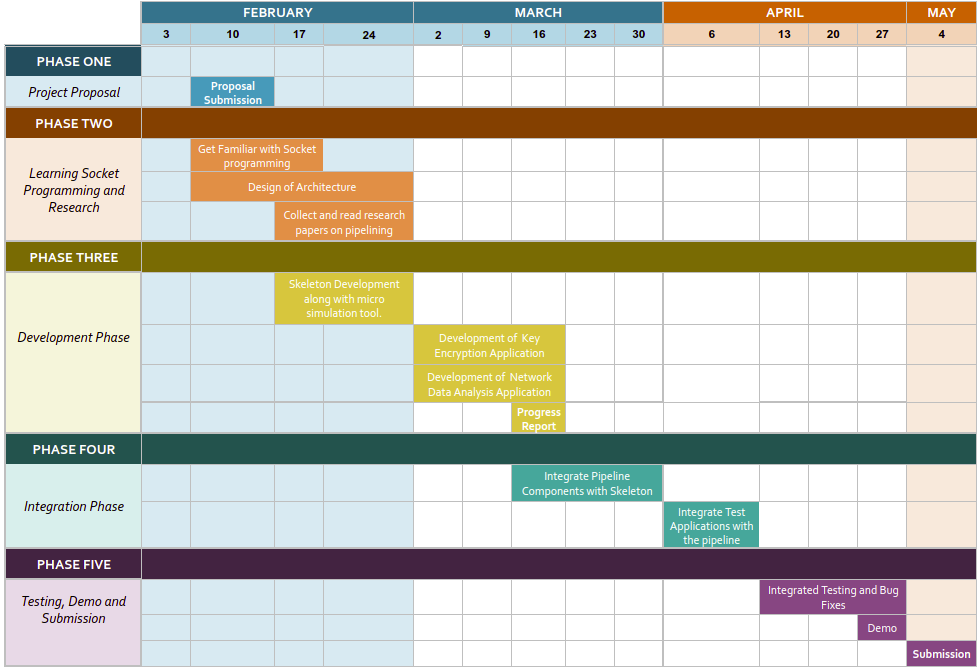
\includegraphics[scale=0.46]{img/timeline.png}
		\label{fig:timeline}
	\end{figure}
}
\newpage
\section*{Test Plan} {
	Testing will be done in two phases.
	\begin{enumerate}
		\item {
			\textbf{Simulation Testing}: In this testing, we will develop a small simulation tool which will run on a single machine and emulate the user, worker and server processes running on separate threads. These threads will communicate with each other using sockets or pipes.
			
			Simulator will be used to test small independent features for unit testing. This will help in increasing the efficiency of the testing. 
			
			\begin{enumerate}
				\item It makes experimenting easy and safe. Development and testing of modules can be done on simulator and once module has been thoroughly tested, it can be directly integrated with the mainline code. 
				\item Developer will not be required to bring up the whole setup every time they want to test the code.
			\end{enumerate}
		}
	
		\item {
			Once all the modules are integrated with the mainline. We will bring up a test bed setup, either in-house or on the cloud. The project will be tested as a singular system for
			
			\begin{enumerate}
				\item All the feature independently.
				
				\item Robustness of the system.
				
				\item Check for security flaws
				
				\item Check for system resource usage such as memory, CPU etc.
			\end{enumerate}
		}
	\end{enumerate}
	
}
